\documentclass[border=0.2cm]{standalone}

% Required package and libraries
\usepackage{tikz}
\usetikzlibrary{decorations.pathmorphing,patterns}

\begin{document}

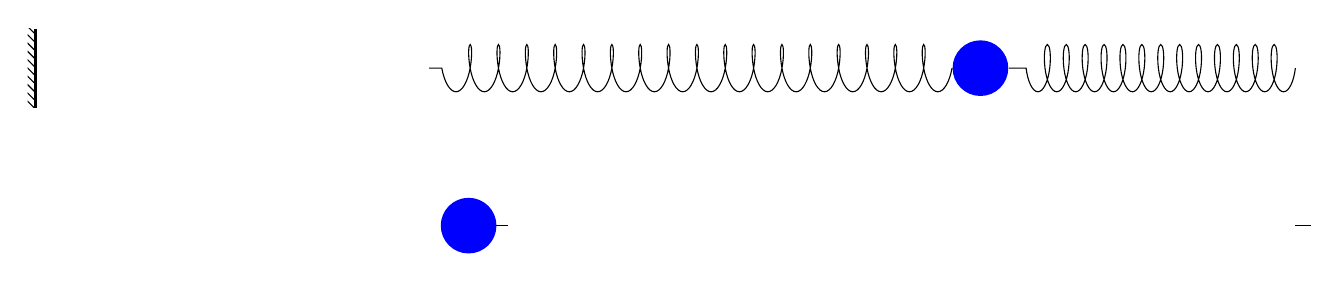
\begin{tikzpicture}


%\draw[pattern=north west lines, pattern color=blue] (0,0) rectangle (2,4);

% Filling a rectangle (solid color)
%\fill[blue] (0,0) rectangle (2,2);

% Filling a circle (solid color)
%\fill[red] (3,0) circle (1cm);

% Filling and drawing a rectangle with an outline
%\filldraw[fill=green, draw=black] (8,0) rectangle (10,2);

% Using a pattern (requires the patterns library)
\usetikzlibrary{patterns}
%\fill[pattern=north east lines] (8,0) rectangle (10,2);

% Using a shading (requires the shadings library)
\usetikzlibrary{shadings}
%\fill[ball color=yellow] (11,0) circle (1cm);



% Left Supporting structure
%		\fill [pattern = north west lines] (-11.1,-.50) rectangle (-11.0,.5);
%		\draw[thick] (-11.0,-.50) -- (-11.0,.50);



%%%%%%%%%%%% Second pattern %%%%%%%%%%%%%%%%%%%

% Left Supporting structure
		\fill [pattern = north west lines] (-11.1,1.50) rectangle (-11.0,2.5);
		\draw[thick] (-11.0,1.50) -- (-11.0,2.50);

%Mass
\node[circle,fill=blue,inner sep=2.5mm] (c) at (1,2.0) {};

%Spring on the right
\draw[decoration={aspect=0.3, segment length=2.4mm, amplitude=3mm,coil},decorate] (5,2.) -- (c); 
\draw[] (5.0,0) -- (5.2,0);
%Spring on the left
%%\draw[decoration={aspect=0.3, segment length=3mm, amplitude=3mm,coil},decorate] (-5,0) -- (a); 
\draw[decoration={aspect=0.3, segment length=3.6mm, amplitude=3mm,coil},decorate] (c) -- (-6,2.0); 
\draw[] (-5.5,0) -- (-5.0,0);
%Mass
\node[circle,fill=blue,inner sep=2.5mm] (b) at (-5.5,0) {};

%\draw[decoration={aspect=0.3, segment length=3mm, amplitude=3mm,coil},decorate] (-6.0,0) -- (-11,0); 
%\draw[] (-6.0,0) -- (-5.5,0);

% Right Supporting structure
%		\fill [pattern = north east lines] (5.2,-.50) rectangle (5.3,.5);
%		\draw[thick] (5.20,-.50) -- (5.20,.50);


\end{tikzpicture}	
\end{document}
